% ! TeX program = pdflatex

\documentclass{article}

\usepackage[a4paper, margin = 1in]{geometry}
\usepackage{listings}
\usepackage{color}

\usepackage{graphicx}
\usepackage{tikz}

\linespread{1.2}

\definecolor{mygreen}{rgb}{0,0.6,0}
\definecolor{mymauve}{rgb}{0.58,0,0.82}

\lstset{
commentstyle=\color{mygreen},
keywordstyle=\color{blue},
stringstyle=\color{mymauve},
identifierstyle=\color{cyan}
}

\newcommand{\code}[1]{\texttt{#1}}

\title
{
	CS420 Compiler Design\\
	Report for the Term Project: Internal Data Structure\\
	${}$\\
	Team 12
}

\author
{
	Jaeseong Choe\\
	Undergraduate\\
	Department of Physics, KAIST
	\and
	Kee Tack Kim\\
	Undergraduate\\
	Department of Mathematics, KAIST
	\and
	Taeyoung Kim\\
	Undergraduate\\
	School of Computing, KAIST
	\and
	Youngrae Kim\\
	Undergraduate\\
	School of Computing, KAIST
	\and
	Seokbin Lee\\
	Undergraduate\\
	School of Computing, KAIST
}

\begin{document}
	\maketitle

	\section{Token}

	The PLY library consist of two \code{.py} files. \code{lex.py} for the lexical analyzer generator and \code{yacc.py} for syntax analyzer generator, respectively. In the \code{lex.py} file, there is special class for tokenization called \code{LexToken}. The \code{LexToken} class has four attributes:

	\begin{itemize}
		\item \code{self.type}
		
		\code{self.type} field represent the type of each token. For example, lexime \code{1234} will has the type \code{ICONST} after it tokenized.

		\item \code{self.value}
		
		\code{self.value} field represent the original string of each token. For example, lexime \code{1234} will has the value '1234' after it tokenized.

		\item \code{self.linno}
		
		\code{self.lino} field represent the line number of each lexime in the source file.

		\item \code{self.lexpos}
		
		\code{self.lexpos} field represent the position of first charactor of each lexime relative to the start of source file.

	\end{itemize}

	\begin{lstlisting}[language=Python, basicstyle = \small]
# Token class.  This class is used to represent the tokens produced.
class LexToken(object):
    def __str__(self):
        return 'LexToken(%s,%r,%d,%d)'
          % (self.type, self.value, self.lineno, self.lexpos)

    def __repr__(self):
        return str(self)
	\end{lstlisting}


	\section{Abstract syntax tree}

	In order to implement abstract syntax tree (AST), we implement the class \code{Node}. The \code{Node} class has two attribute:

	\begin{itemize}
		\item \code{self.data}
		
		\code{self.data} is an identifier to represent general data contained in node. The type of data can be anything. The beauty of Python!

		\item \code{self.children}
		
		\code{self.children} is a list which contains the children of node.

	\end{itemize}

	\section{Symbol table}
	Symbol table is constructed by symbol table block, and consequentluy it is consist of symbol table entries. We make not only the symbol table, but also the symbol table block since we have to handle the scope of variables. Symbol Table blocks are connected as rooted tree.

	Figure \ref{fig:SymTab} is a diagram of example of symbol table. The big blue rectangle represents the symbol table class, and an arrow shows \code{self.cur} of symbol table. Each gray rectangle represents symbol table blocks, and blocks stores information of symbols.

	\begin{itemize}
		\item \code{self.id} in \code{SymTabEntry} class
		
		\code{self.id} stores identifier's name.
		
		\item \code{self.type} in \code{SymTabEntry} class
		
		\code{self.id} stores identifier's type.
		
		\item \code{self.assigned} in \code{SymTabEntry} class
		
		If this identifier is assigned with some value, then \code{self.assigned} is \code{True}. If not, then \code{False}.

		\item \code{self.prev} in \code{SymTabBlock} class
		
		\code{self.prev} shows the parent block.

		\item \code{self.next} in \code{SymTabBlock} class
		
		\code{self.next} is a list of children blocks.

		\item \code{self.table} in \code{SymTabBlock} class
		
		\code{self.table} contains actual information of symbols. It is a dictionary type which is consist of instances of \code{SymTabEntry} class.

		\item \code{self.cur} in \code{SymTab} class
		
		\code{self.cur} represents the specific symbol table block. There are several methods to insert or remove symbols into \code{self.cur} block.
	\end{itemize}

	\begin{lstlisting}[language=Python, basicstyle = \footnotesize]
# Symbol table entry class. This class is used
# to represent the entries of symbol table block.
class SymTabEntry:
    def __init__(self, id, type, assigned=False):
        self.id = id
        self.type = type
        self.assigned = assigned


class SymTabBlock:
    def __init__(self, prev=None, nexts=[]):
        self.prev = prev
        self.nexts = nexts
        self.table = {}

    def insert(self, symbol):
        if symbol.id in self.table:
            # Need to implement (maybe try-except?)
            pass
        else:
            self.table[symbol.id] = symbol

    def remove(self, id):
        if id not in self.table.keys():
            # Need to implement (maybe try-except?)
            pass
        else:
            self.table.pop(id)

    def get(self, id):
        try:
            return self.table[id]
        except KeyError:
            # Need to implement
            pass


class SymTab:
    def __init__(self):
        global_table = SymTabBlock(None)
        self.cur = global_table

    def insert_block_table(self, block_table):
        self.cur.nexts.append(block_table)
        block_table.prev = self.cur
        self.cur = block_table

    def remove_block_table(self):
        self.cur.prev.pop(self.cur)
        self.cur = self.cur.prev
        
    def insert(self, symbol):
        self.cur.insert(symbol)

    def remove(self, id):
        self.cur.remove(id)

    def get(self, id):
        table = self.cur
        while table != None:
            entry = table.get(id)
            if entry != None:
                table = table.prev
            else:
                return entry
        return None
	\end{lstlisting}


	\section{Intermediate code}
	We decided that to use triplet to represent intermediate code. It will be expressed by list of ordered triples.

	%%%%%%%%%%%%%%%%%%%%%%%%%%%%%%%%%%%% Figures

	\begin{figure}[ht]
		\centering
		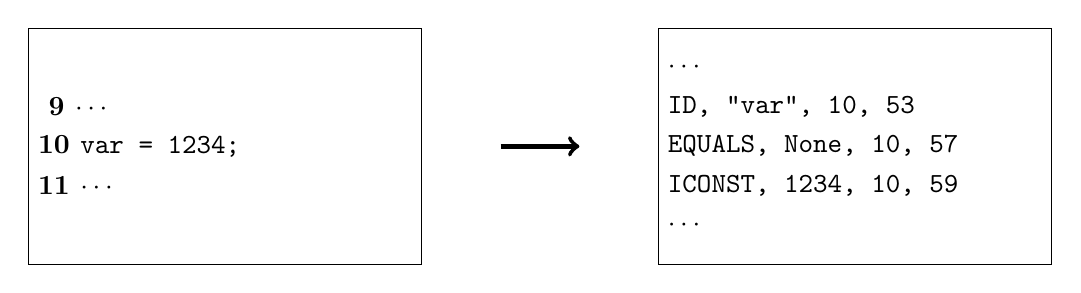
\begin{tikzpicture}
			\draw (0,3.5) rectangle (5,0.5);
			\draw (0,2.5) node[anchor=west] {\textbf{ 9 }\code{$\cdots$}};
			\draw (0,2) node[anchor=west] {\textbf{10 }\code{var = 1234;}};
			\draw (0,1.5) node[anchor=west] {\textbf{11 }\code{$\cdots$}};

			\draw[->, ultra thick] (6,2) -- (7,2);

			\draw (8,3.5) rectangle (13,0.5);
			\draw (8,3) node[anchor=west] {\code{$\cdots$}};
			\draw (8,2.5) node[anchor=west] {\code{ID, "var", 10, 53}};
			\draw (8,2) node[anchor=west] {\code{EQUALS, None, 10, 57}};
			\draw (8,1.5) node[anchor=west] {\code{ICONST, 1234, 10, 59}};
			\draw (8,1) node[anchor=west] {\code{$\cdots$}};

		\end{tikzpicture}
		\caption{Figure of tokenization. This shows that translation of source code to list of tokens.}
		\label{fig:token}
	\end{figure}

	\begin{figure}[ht]
		\centering
		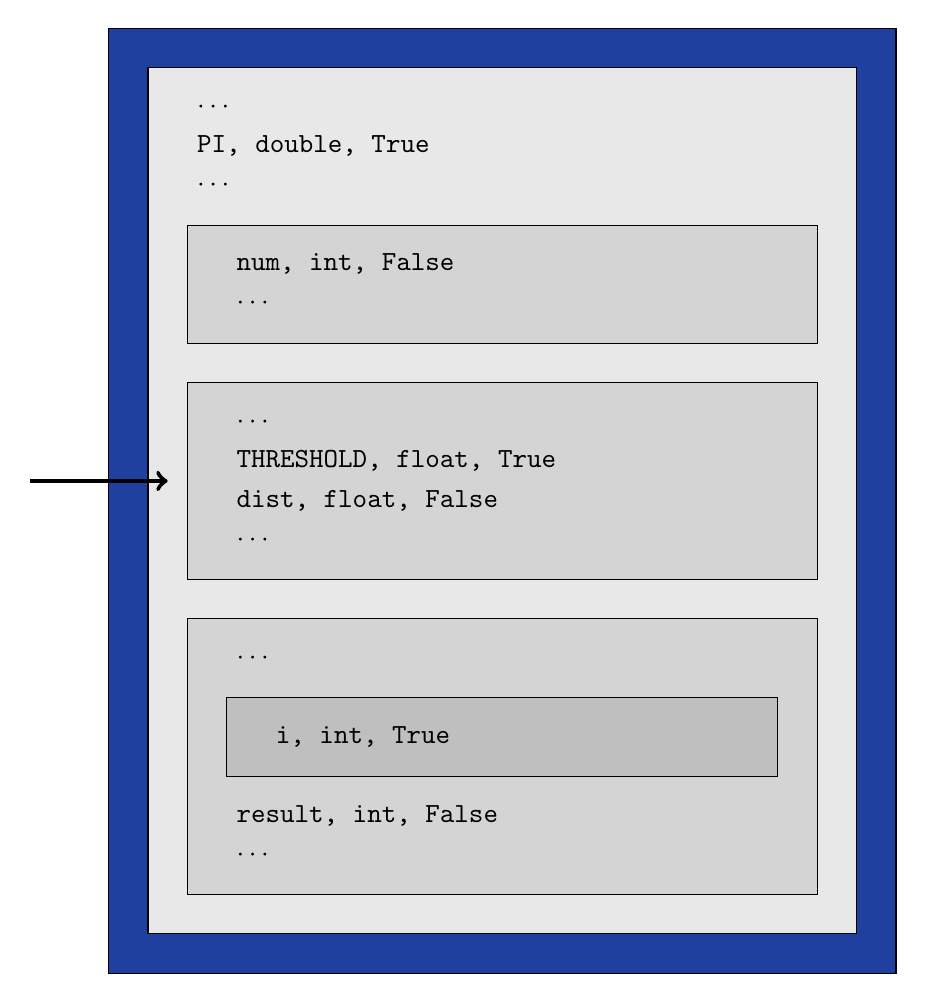
\begin{tikzpicture}
			\draw[fill={rgb:red,1;green,2;blue,5}] (0,0) rectangle (10, 12);

			\draw[fill={rgb:black,1;white,10}] (0.5,0.5) rectangle (9.5, 11.5);
			
			\draw[fill={rgb:black,1;white,5}] (1,1) rectangle (9, 4.5);
			\draw[fill={rgb:black,1;white,5}] (1,5) rectangle (9, 7.5);
			\draw[fill={rgb:black,1;white,5}] (1,8) rectangle (9, 9.5);
			
			\draw[fill={rgb:black,1;white,3}] (1.5,2.5) rectangle (8.5, 3.5);

			
			\draw (1,11) node[anchor=west] {\code{$\cdots$}};
			\draw (1,10.5) node[anchor=west] {\code{PI, double, True}};
			\draw (1,10) node[anchor=west] {\code{$\cdots$}};
			
			\draw (1.5,9) node[anchor=west] {\code{num, int, False}};
			\draw (1.5,8.5) node[anchor=west] {\code{$\cdots$}};

			\draw (1.5,7) node[anchor=west] {\code{$\cdots$}};
			\draw (1.5,6.5) node[anchor=west] {\code{THRESHOLD, float, True}};
			\draw (1.5,6) node[anchor=west] {\code{dist, float, False}};
			\draw (1.5,5.5) node[anchor=west] {\code{$\cdots$}};

			\draw (1.5,4) node[anchor=west] {\code{$\cdots$}};
			\draw (2,3) node[anchor=west] {\code{i, int, True}};
			\draw (1.5,2) node[anchor=west] {\code{result, int, False}};
			\draw (1.5,1.5) node[anchor=west] {\code{$\cdots$}};

			
			\draw[->, ultra thick] (-1,6.25) -- (0.75,6.25);
		\end{tikzpicture}
		\caption{Symbol Table structure.}
		\label{fig:SymTab}
	\end{figure}

\end{document}